\documentclass{standalone}
\usepackage{tikz}
\usepackage{ctex,siunitx}
\usepackage{tkz-euclide}
\usepackage{amsmath}
\usetikzlibrary{patterns, calc}
\usetikzlibrary {decorations.pathmorphing, decorations.pathreplacing, decorations.shapes,}
\begin{document}
\small
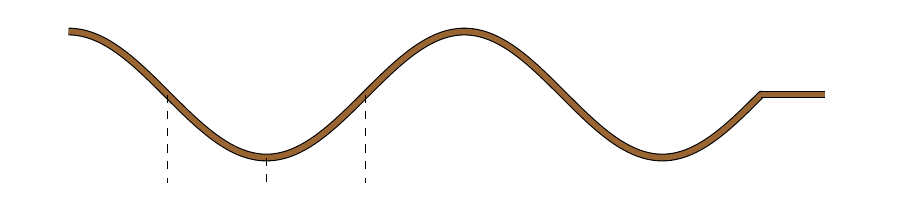
\begin{tikzpicture}[>=stealth, scale=0.8, domain=0:3.5*pi, samples=200]
  \draw [->,draw=none](0,0)node [left]{$\phantom{O}$}--(12.5,0) node [below]{$\phantom{x}$};
  \draw[fill=brown!80!black](3.5*pi,0)circle(1.5pt);
  \draw [double=brown!80!black,double distance=2pt, domain=0:3.5*pi]  plot (\x,{cos(\x r)});
  \draw [double=brown!80!black,double distance=2pt, domain=3.5*pi:12]  plot (\x,0);
  \draw [dashed](.5*pi, 0) -- (.5*pi, -1.4);  
  \draw [dashed](pi,-1) -- (pi, -1.4);  
  \draw [dashed](1.5*pi, 0) -- (1.5*pi,-1.4);     
\end{tikzpicture}
\end{document}